% Diese Zeile bitte -nicht- aendern.
\documentclass[course=erap]{aspdoc}

%%%%%%%%%%%%%%%%%%%%%%%%%%%%%%%%%
\newcommand{\theGroup}{110}
\newcommand{\theNumber}{A201}
\author{Simon Bußmann \and Nico Lintner \and Manuel Walter Mußbacher}
\date{Sommersemester 2023}
%%%%%%%%%%%%%%%%%%%%%%%%%%%%%%%%%

% Diese Zeile bitte -nicht- aendern.
\title{Gruppe \theGroup{} -- Abgabe zu Aufgabe \theNumber}

\usepackage{caption}
\usepackage{subcaption}

\begin{document}
\maketitle

\section{Einleitung}

In diesem Projekt haben wir uns damit beschäftigt, den Sobel-Filter Algorithmus zu implementieren.
Dieser Algorithmus wird verwendet, um Kanten in Bildern zu erkennen.
Dabei werden die Pixel eines Bildes mit zwei Matritzen, sogenannte Filter, verrechnet.
Die aus dieser Verrechnung resultierenden Werte werden dann in einem neuen Bild gespeichert.
\begin{figure}[H]
    \begin{subfigure}{.5\columnwidth}
        \centering
        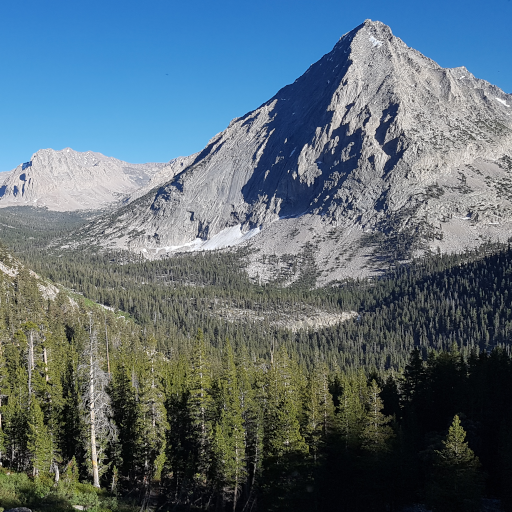
\includegraphics[width=\columnwidth]{graphics/johnmuirtrail.png}
        \caption{Input-Bild}
        \label{fig:input-bild}
    \end{subfigure}
    \begin{subfigure}{.5\columnwidth}
        \centering
        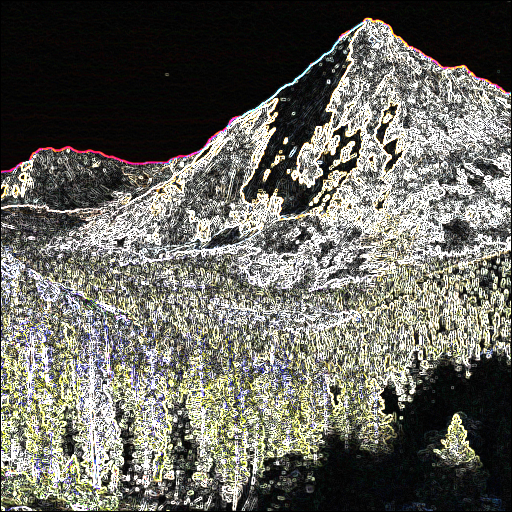
\includegraphics[width=\columnwidth]{graphics/johnmuirtrail_sobel.png}
        \caption{Output-Bild}
        \label{fig:output-bild}
    \end{subfigure}
\end{figure}

In Abbildung \ref{fig:input-bild} und \ref{fig:output-bild} ist ein Beispiel für die Anwendung des Sobel-Filters zu sehen.

\section{Lösungsansatz}

Unser gewählter Lösungsansatz besteht aus drei verschiedenen Versionen:
Die erste Version implementiert den Sobel-Filter strikt nach seiner mathematischen Definition (src zu Aufgabenstellung).
Diese Version dient zusätzlich als Vergleichsimplementierung.
Die zweite und dritte Version bauen jeweils aufeinander auf und zielen darauf ab, die Laufzeit der ersten, naiven Version bedeutend zu verbessern;
Version Zwei verwendet Single Instruction Multiple Data (SIMD) Instruktionen, um eine größere Bandweite bei der Berechnung des Filters zu erreichen.
Dabei werden die Farbwerte von mehr als 5 Pixeln simultan berechnet und gespeichert.
Version Drei kombiniert besagte erhöhte Bandbreite mit Multithreading, um die hohe Parallelität moderner Prozessoren optimal auszunutzen.
Alle Implementierungen arbeiten mit 24-Bit BMP-Bildern.
Ein Pixel besteht dabei aus drei Bytes, die die Farbwerte für Blau, Grün und Rot repräsentieren.

\subsection{Vergleichsimplementierung}
\label{sec:vergleichsimplementierung}
Die Vergleichsimplementierung ist eine naive Implementierung des Sobel-Filter Algorithmus.
Dabei werden die beiden Filtermatritzen $M^{v}$ und $M^{h}$ mit jedem Pixel des Bildes verrechnet.
\begin{equation}
    M^{v} :
    \begin{bmatrix}
        1 & 0 & -1 \\
        2 & 0 & -2 \\
        1 & 0 & -1
    \end{bmatrix}
    M^{h} :
    \begin{bmatrix}
        1 & 2 & 1 \\
        0 & 0 & 0 \\
        -1 & -2 & -1
    \end{bmatrix}
\end{equation}
\begin{equation}
    A^{h} = M^{h} * Image
\end{equation}
\begin{equation}
    A^{v} = M^{v} * Image
\end{equation} \\
Für Kantenerkennung macht es nur Sinn, die drei Farbkanäle F eines jeden Pixels mit Koordinaten (x, y) im Eingabebild B separat zu betrachten.
Um die Farbinformationen für die vertikalen bzw. horizontalen Kanten in einem Ausgabebild B zu berechnen, wird der entsprechende Farbkanal jedes umittelbar umliegenden Pixels in B mit dem dazugehörigen Wert der Filtermatritzen (Mv und Mh respektive) multipliziert und die Produkte anschließend aufsummiert.
Pixel, die sich am Rand des Bildes befinden, können nicht mit allen Werten der Filtermatritzen verrechnet werden.
Dieser Fall wird behandelt, indem die Sobelwerte dieser Pixel nicht berechnet werden.
Hierdurch entsteht implizit ein schwarzer Rand um das Bild.
\begin{equation}
    A_(x,y)^{v,F} = \sum_{i=-1}^{1} \sum_{j=-1}^{1} M^{v}_{i,j} * B_{(x+i,y+j)}^{F}
\end{equation}
\begin{equation}
    A_(x,y)^{h,F} = \sum_{i=-1}^{1} \sum_{j=-1}^{1} M^{h}_{i,j} * B_{(x+i,y+j)}^{F}
\end{equation}
Um nun den Sobelwert O für einen Farbkanal eines Pixels zu berechnen, werden die Beträge des entsprechenden Farbkanals des dazugehörigen Pixels der vertikalen und horizontalen Kanten addiert.
\begin{equation}
    O^{F}_{x,y} = \left | A^{v,F}_{x,y} \right | + \left | A^{h,F}_{x,y} \right |
    \label{eq:betrag}
\end{equation}

\label{sec:rand}
\\\\
Alternativ kann im letzten Schritt der endgültige Sobelwert analog mit der Wurzel aus der Summe der Quadrate berechnet.
\begin{equation}
    O^{F}_{x,y} = \sqrt{(A^{v,F}_{x,y})^2 + (A^{h,F}_{x,y})^2}
    \label{eq:wurzel}
\end{equation}
\begin{figure}[H]
    \begin{subfigure}{.5\columnwidth}
        \centering
        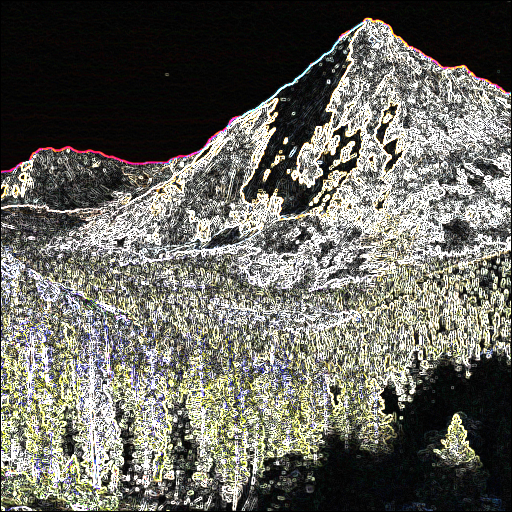
\includegraphics[width=\columnwidth]{graphics/johnmuirtrail_sobel.png}
        \caption{Abs Version \ref{eq:betrag}}
        \label{fig:abs-bild}
    \end{subfigure}
        \begin{subfigure}{.5\columnwidth}
        \centering
        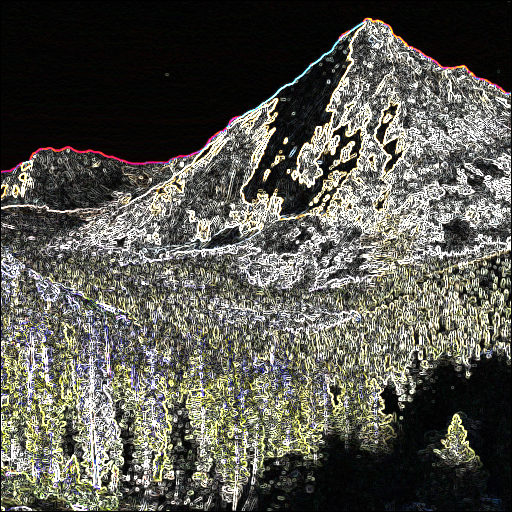
\includegraphics[width=\columnwidth]{graphics/sqrt_sobel.png}
        \caption{Sqrt Version \ref{eq:wurzel}}
        \label{fig:sqrt-bild}
    \end{subfigure}
\end{figure}
Zwischen {\ref{fig:abs-bild}} und {\ref{fig:sqrt-bild}} besteht nur ein kleiner Unterschied in der Helligkeit des Bildes, was für Kantenerkennung nicht relevant ist.
Da keine SIMD-Instruktion zur Berechnung der Wurzel eines 8 bzw. 16 Bit Integers existiert und diese Version als Vergleichsimplementierung genutzt werden soll, haben wir uns für die Variante {\ref{eq:betrag}} entschieden.
\subsection{SIMD Implementierung}
\label{sec:simd-implementierung}
Die SIMD Implementierung basiert auf der Vergleichsimplementierung, benutzt zur Berechnung jedoch SIMD Instruktionen.
Ein großes Problem bei der Arbeit mit 8-Bit-Ganzzahlen ist der kleine Wertebereich.
Da die Werte der einzelnen Farbchannel der Pixel als 8 Bit Integer gespeichert werden, kann es folglich bei der Faltungsoperation schnell zu einem Überlauf kommen.
Der naive Lösungsansatz, um dem entgegen zu wirken, ist das Input-Bild schlicht um 75\% zu verdunkeln.
Durch die Verdunkelung wird der Überlauf zwar verhindert, das Output Bild ist jedoch auch (wesentlich) dunkler {\ref{fig:dark}}, wodurch die erkannten Kanten signifikant dunkler werden.
\begin{figure}[H]
    \begin{subfigure}{.5\columnwidth}
        \centering
        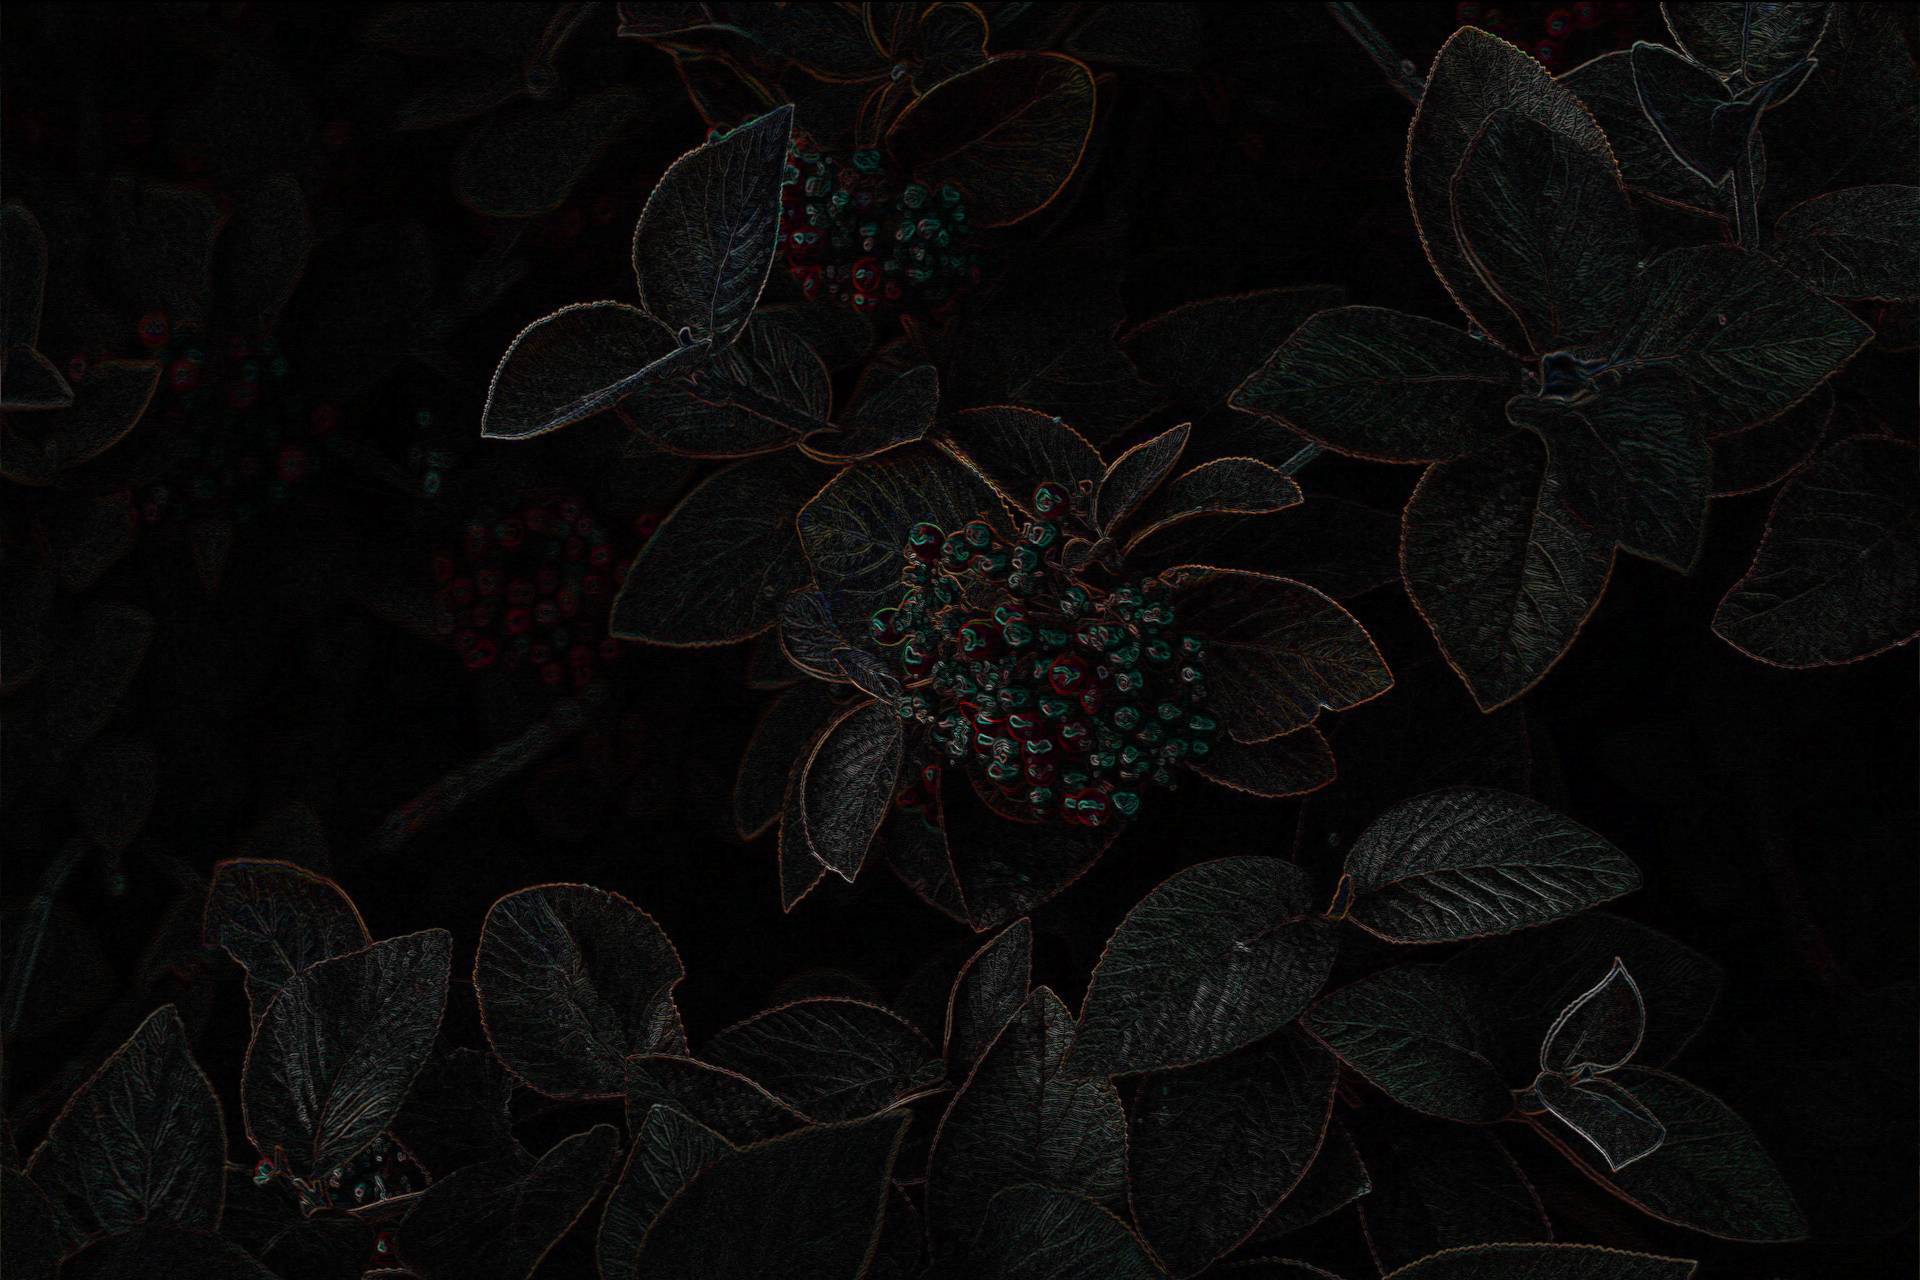
\includegraphics[width=\columnwidth]{graphics/dark.png}
        \caption{Erste SIMD Version}
        \label{fig:dark}
    \end{subfigure}
    \begin{subfigure}{.5\columnwidth}
        \centering
        \includegraphics[width=\columnwidth]{graphics/correct.png}
        \caption{Vergleichsimplementierung}
        \label{fig:correct}
    \end{subfigure}
\end{figure}
Um trotz Vektorinstruktionen und sehr kleinen Wertebereichen ein Ergebnis zu erzielen,
das exakt der Vergleichsimplementierung entspricht, werden die Daten aus einem 16-Byte-Speicherbereich so in zwei Vektoren geladen, dass während der Berechnung je 8 Byte
als 16-Bit-Integer interpretiert werden können.
Dabei werden insgesamt 16 xmm Register benutzt, um jeweils die Sobel Werte für 16 Farbchannel gleichzeitig zu berechnen.
Das funktioniert so, dass ein 16 Byte-Speicherbereich gelesen wird und anschließend das jeweils höherwertige Byte eines jeden
16-Bit-Integers in diesem Vektor mit einer Bitmaske genullt wird.
Das geschieht analog mit den 16-Byte an der um einen Byte höheren Speicheradresse.
Für jeden der 16 Farbchannel, die mit einem Schleifendurchlauf berechnet werden können, werden so die acht umliegenden Farbchannel geladen.
Durch den entstehenden Overhead ist dieser Lösungsansatz zwar ca. nur halb so schnell, wie der naive SIMD-Ansatz, erzeugt jedoch ein korrektes Ergebnis, weshalb das Programm auch diesen Ansatz implementiert.

\subsection{SIMD-Implementierung mit Threading}
\label{sec:simd-threading}
Die SIMD-Implementierung mit Threading basiert auf der SIMD-Implementierung mit der Besonderheit, dass das Bild in Abschnitte eingeteilt werden, die jeweils von einem eigenen Thread bearbeitet werden.
Um diese Abschnitte zu erzeugen, wird das Bild in horizontale Streifen geschnitten.
Die Anzahl der Streifen wird von der Anzahl der durch die CPU bereitgestellten Threads bestimmt.
Dies führt zu einer Optimalen Auslastung der CPU.
Das horizontale Zerteilen des Bildes hat den Vorteil, dass der Cache besser genutzt wird, als zum Beispiel beim Aufteilen in Quadranten, weil die Daten hintereinander Zeile für Zeile im Speicher liegen.
Desweiteren besteht der Vorteil, fortlaufende Indizes bei der Berechnung nutzen zu können und nicht, wie zum Beispiel bei einer Aufteilung in Quadranten, diese Indizes aufwendig berechenen zu müssen.

\section{Genauigkeit}
Im folgenden wird die Genauigkeit unseres Lösungsansatzes analysiert, da es beim Sobel Operator keine fest definierte "source of truth", wie zum Beispiel bei einer Addition, gibt.
Die öffentlich existierende Sobel-Filter Implementierung von OpenCV liefert beispielsweise Ergebnisse, die sich leicht in der Helligkeit von unserer unterscheiden.
Desweiteren arbeitet diese auf Graustufenbildern, wohingegen unsere Implementierung auf RGB-Bildern arbeitet.
Wir haben die Implementierung von OpenCV so angepasst, dass sie ebenfalls auf RGB-Bildern arbeiten kann, um die Ergebnisse mit unseren zu vergleichen.
\begin{figure}[H]
    \begin{subfigure}{.5\columnwidth}
        \centering
        \includegraphics[width=\columnwidth]{graphics/basic.png}
        \caption{Vergleichsimplementierung}
        \label{fig:basic}
    \end{subfigure}
    \begin{subfigure}{.5\columnwidth}
        \centering
        \includegraphics[width=\columnwidth]{graphics/open_cv.png}
        \caption{Open CV Version}
        \label{fig:opencv}
    \end{subfigure}
\end{figure}
In {\ref{fig:basic}} ist die Vergleichsimplementierung zu sehen, in {\ref{fig:opencv}} die OpenCV Implementierung.
Es ist zu erkennen, dass die OpenCV Implementierung wesentlich dunkler (~50\%) ist als die Vergleichsimplementierung.
Da die Kanten dennoch korrekt (!und kontrastreicher!) erkannt werden und um unnötige Rechenschritte zu vermeiden, wird die Helligkeit der Vergleichsimplementierung nicht angepasst.
\\\\
Bei der Bewertung der Genauigkeit wird die Vergleichsimplementierung als Referenzpunkt verwendet.
Sie gilt als das korrekte Ergebnis und ist, um Fehler zu vermeiden, so simpel und leserlich gehalten wie nur irgendwie möglich.
Die mathematische Defintion, wie in \ref{sec:vergleichsimplementierung} beschrieben, wurde ohne weitere Optimierungen umgesetzt.
Des weiteren wurden Unittests hinzugefügt, die überprüfen, ob die Hilfsfunktionen korrekt implementiert sind.
Die optimierten Versionen SIMD \ref{sec:simd-implementierung} und SIMD mit Threading \ref{sec:simd-threading} erzielen Ergebnisse, die denen der Verlgiechimplementierung exakt entsprechen.
Um das zu erreichen, wird der in Version 1 implizit entstehende schwarze Rand explizit links und rechts nach der Berechnung hinzugefügt.
Da dafür - für Bilder mit herkömmlicher Größe - verschwindend wenig Schreiboperationen benötigt werden ist die Perfromanzeinbuße kaum messbar.
\\\\
*TODO: Performance overhead zeigen*
\\\\
Es gibt außerdem einen automatisierten Test, der überprüft ob die Ergebnisse der SIMD und SIMD + Threading Versionen mit den
Ergebnissen der Vergleichsimplementierung übereinstimmen.

\section{Performanzanalyse}

TODO: Geben Sie hier die Performanz Ihres Lösungsansatzes ein.

\section{Zusammenfassung und Ausblick}

TODO: Geben Sie hier eine kurze Zusammenfassung und einen Ausblick ein.

% TODO: Fuegen Sie Ihre Quellen der Datei Ausarbeitung.bib hinzu
% Referenzieren Sie diese dann mit \cite{}.
% Beispiel: CR2 ist ein Register der x86-Architektur~\cite{intel2017man}.
\bibliographystyle{plain}
\bibliography{Ausarbeitung}

\end{document}
